%%%%%%%%%%%%%%%%%%%%%%%%%%%%%%%%%%%%%%%%%%%%%%%%%%%%%%%%%%%%%%%%%%%%%%%%%%%%%%%%%%%%%%%%%%%%%%%%%
% Chapter 3: Methodology   (the \chapter command is in main.tex)
%%%%%%%%%%%%%%%%%%%%%%%%%%%%%%%%%%%%%%%%%%%%%%%%%%%%%%%%%%%%%%%%%%%%%%%%%%%%%%%%%%%%%%%%%%%%%%%%%

%--------------------------------------------------------------------------------------------------
\section{System overview}\label{sec:m_overview}
%--------------------------------------------------------------------------------------------------

Figure~\ref{fig:m_system} shows the system. The simulator flies the drone and computes the true battery state. The sensors turn the true current and voltage into imperfect readings. The EKF and the two baselines (charge counting and a voltage threshold) see only these readings, and each feeds a turn-back decision. Only the simulator knows the truth, so every estimate and every decision can be scored exactly.

\label{sec:m_assumptions}The drone carries a six-cell series lithium-ion pack of 5\,Ah. The same current flows through every cell, so one cell is modelled; all voltages and battery parameters are per cell. Everything runs once per second ($\Delta t = 1$\,s); $I_k$ is the current during step $k$ and every state with index $k$ is its value at the end of that step.

\begin{figure}[htbp]
  \centering
  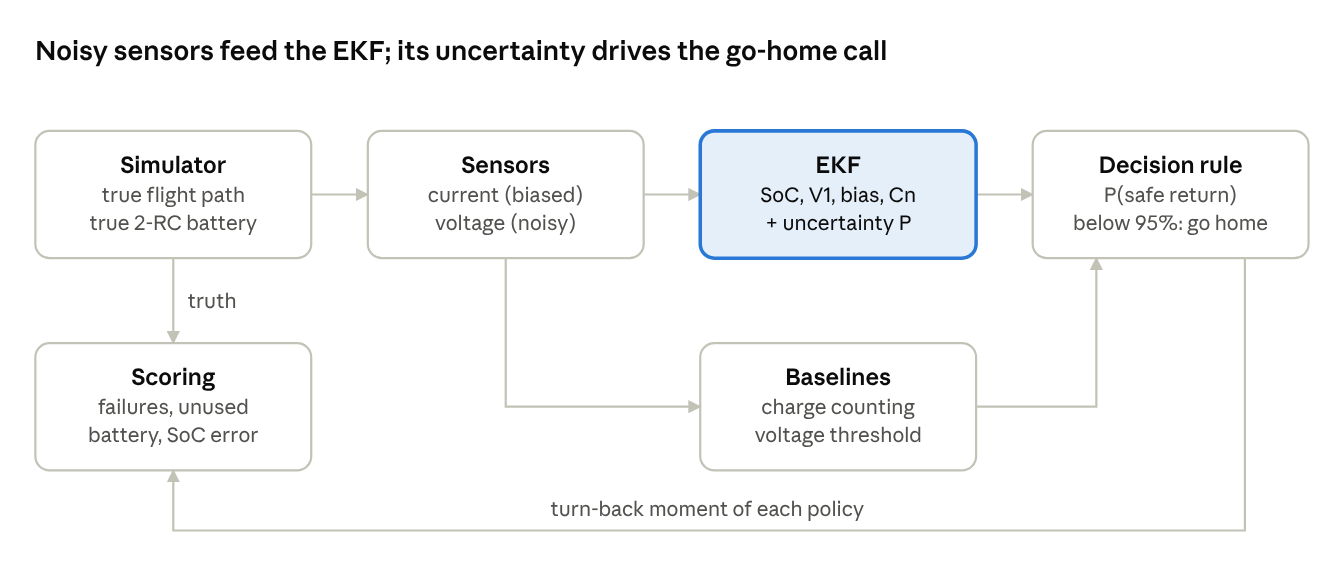
\includegraphics[width=\textwidth]{fig1_system_overview.png}
  \caption[System overview.]{System overview. The EKF and the baselines see only the noisy sensor readings; the simulator's truth is used only for scoring. (The EKF block lists four states; the final filter also learns $R_0$, Section~\ref{sec:m_ekf_stages}.)}
  \label{fig:m_system}
\end{figure}

%--------------------------------------------------------------------------------------------------
\section{Battery models: truth versus filter}\label{sec:m_truth_vs_filter}
%--------------------------------------------------------------------------------------------------

A filter tested against its own model always looks good, and a real filter never has the exact model. The simulated battery is therefore deliberately different from the filter's model (Table~\ref{tab:m_params}).

\label{sec:m_rc_discrete}\label{sec:m_truth}With the current held constant during a step, an RC pair \eqref{eq:bg_rc} updates exactly as
\begin{equation}
  V_{i,k} = a_i\, V_{i,k-1} + R_i\,(1 - a_i)\, I_k, \qquad a_i = e^{-\Delta t / (R_i C_i)} .
  \label{eq:m_rc_discrete}
\end{equation}
The true battery has a second, slow RC pair ($R_2$, $C_2$) that the filter does not know about, and an OCV curve shifted by $\delta_{\text{OCV}}$:
\begin{align}
  \mathrm{SoC}_k &= \mathrm{SoC}_{k-1} - \frac{I_k\, \Delta t}{3600\, C_n}, \qquad V_{1,k},\, V_{2,k} \text{ from \eqref{eq:m_rc_discrete}}, \label{eq:m_true_soc}\\
  V_k &= \mathrm{OCV}(\mathrm{SoC}_k) + \delta_{\text{OCV}} - R_0\, I_k - V_{1,k} - V_{2,k}. \label{eq:m_true_v}
\end{align}
The battery is dead if $V_k < 3.0$\,V while current flows.

\label{sec:m_ocv}Both models use the same representative lithium-ion OCV table (Figure~\ref{fig:bg_ocv_tangent}), smoothed with shape-preserving cubic interpolation (\texttt{pchip}) so its slope does not jump. The EKF needs the slope, found by a central difference over $\pm 0.5\%$ SoC (one-sided at the ends of the table):
\begin{equation}
  \frac{d\,\mathrm{OCV}}{d\,\mathrm{SoC}}(s) \approx \frac{\mathrm{OCV}(s^{+}) - \mathrm{OCV}(s^{-})}{s^{+} - s^{-}}, \qquad s^{\pm} = s \pm 0.005 .
  \label{eq:m_ocv_slope}
\end{equation}

\begin{table}[htbp]
  \centering
  \caption{Battery parameters per cell (\texttt{config/battery\_params.m}).}
  \label{tab:m_params}
  \begin{tabular}{@{}lccl@{}}
    \toprule
    Parameter & Filter & Truth & Note \\
    \midrule
    Circuit & 1 RC pair & 2 RC pairs & \\
    $C_n$ & 5.0\,Ah & 5.0\,Ah & 4.25\,Ah in E4 \\
    $R_0$ & 8\,m$\Omega$ & 8.8\,m$\Omega$ & +10\% \\
    $R_1$, $C_1$ & 6\,m$\Omega$, 5000\,F & 5.4\,m$\Omega$, 5500\,F & $\tau_1 \approx 30$\,s \\
    $R_2$, $C_2$ & -- & 1.5\,m$\Omega$, 266\,667\,F & $\tau_2 = 400$\,s; 4\,m$\Omega$ in E6 \\
    $\delta_{\text{OCV}}$ & 0 & $-5$\,mV & \\
    \bottomrule
  \end{tabular}
\end{table}

\label{sec:m_params}\label{sec:m_why_mismatch}The slow pair is the most visible difference: with $\tau_2 = 400$\,s its voltage keeps building through most of a 15-minute flight, and the filter has no state for it. A first setting, $R_2 = 4$\,m$\Omega$, was used for the simulator test (Section~\ref{sec:r_sim}); at 15\,A it adds about 63\,mV of unmodelled drop, which on the flat part of the curve looks like up to 13\% SoC error. That is harsher than a reasonably identified model, so the default was reduced to 1.5\,m$\Omega$ (about 23\,mV) and the strong setting kept as stress test E6.

%--------------------------------------------------------------------------------------------------
\section{Sensors and mission}\label{sec:m_sensors}\label{sec:m_mission}
%--------------------------------------------------------------------------------------------------

The sensors read
\begin{equation}
  I_{m,k} = I_k + b + w_{I,k}, \qquad V_{m,k} = V_k + v_k,
  \label{eq:m_sensor_i}
\end{equation}
with a current bias $b$ (0.5\,A by default), current noise $\sigma_I = 0.2$\,A and voltage noise $\sigma_V = 10$\,mV.

The drone takes off (30\,s at 30\,A), cruises at 10\,m/s to each drop-off ($15\,\text{A} \times (1+w)$, where $w$ is a wind factor), hovers 30\,s at 20\,A to deliver, flies home and lands (40\,s at 18\,A). A slowly varying random load is added while flying:
\begin{equation}
  \varepsilon_k = 0.9\,\varepsilon_{k-1} + 0.3\, n_k, \quad n_k \sim \mathcal{N}(0, 1), \qquad I_k = \max(I_{\text{demand},k} + \varepsilon_k,\, 0),
  \label{eq:m_wobble}
\end{equation}
which wanders by about $\pm 0.7$\,A. The \emph{short} route has three drop-offs and ends with charge to spare; the \emph{long} route has six drop-offs reaching 9\,km and is too far for one battery, so the return-to-home rule must act.

%--------------------------------------------------------------------------------------------------
\section{The Extended Kalman Filter}\label{sec:m_ekf}
%--------------------------------------------------------------------------------------------------

\subsection{Model}\label{sec:m_ekf_states}\label{sec:m_ekf_process}\label{sec:m_ekf_measurement}

The state, input and measurement are
\begin{equation}
  x_k = \begin{bmatrix} \mathrm{SoC}_k & V_{1,k} & b_k & C_{n,k} & R_{0,k} \end{bmatrix}^{\top}, \qquad u_k = I_{m,k}, \qquad z_k = V_{m,k}.
  \label{eq:m_state}
\end{equation}
The filter's best guess of the true current is $I_{m,k} - b$. The process model is charge counting and the RC update with this corrected current, while the bias, capacity and resistance are treated as constants that may wander slowly (this is how a filter learns an unknown constant):
\begin{align}
  \mathrm{SoC}_k &= \mathrm{SoC}_{k-1} - \frac{(I_{m,k} - b_{k-1})\, \Delta t}{3600\, C_{n,k-1}}, \label{eq:m_f_soc}\\
  V_{1,k} &= a\, V_{1,k-1} + R_1 (1 - a)(I_{m,k} - b_{k-1}), \label{eq:m_f_v1}\\
  b_k &= b_{k-1} + w_b, \qquad C_{n,k} = C_{n,k-1} + w_C, \qquad R_{0,k} = R_{0,k-1} + w_R. \label{eq:m_f_r0}
\end{align}
The measurement model is the circuit equation \eqref{eq:bg_terminal}:
\begin{equation}
  V_{m,k} = \mathrm{OCV}(\mathrm{SoC}_k) - V_{1,k} - R_{0,k}\,(I_{m,k} - b_k) + v_k .
  \label{eq:m_h}
\end{equation}

\subsection{Jacobians}\label{sec:m_ekf_f}\label{sec:m_ekf_h}

Differentiating \eqref{eq:m_f_soc}--\eqref{eq:m_h} with respect to the state gives
\begin{equation}
  F_k =
  \begin{bmatrix}
    1 & 0 & \frac{\Delta t}{3600\, \hat{C}_n} & \frac{(I_m - \hat{b})\, \Delta t}{3600\, \hat{C}_n^{2}} & 0 \\[3pt]
    0 & a & -R_1 (1 - a) & 0 & 0 \\
    0 & 0 & 1 & 0 & 0 \\
    0 & 0 & 0 & 1 & 0 \\
    0 & 0 & 0 & 0 & 1
  \end{bmatrix},
  \qquad
  H_k^{\top} =
  \begin{bmatrix} d\,\mathrm{OCV}/d\,\mathrm{SoC} \\ -1 \\ \hat{R}_0 \\ 0 \\ -(I_m - \hat{b}) \end{bmatrix}.
  \label{eq:m_F}
\end{equation}
The OCV slope makes the voltage correct the SoC strongly near empty and weakly in the flat middle. The resistance entry grows with the current, so the resistance shows up most when the current changes. The capacity entry of $H$ is zero: capacity is learned only slowly, through how the SoC drifts.

\subsection{Noise}\label{sec:m_ekf_q}

The current-sensor noise enters the prediction through
\[
  G_k = \frac{\partial f}{\partial I_m} = \begin{bmatrix} -\frac{\Delta t}{3600\, \hat{C}_n} & R_1(1-a) & 0 & 0 & 0 \end{bmatrix}^{\top}.
\]
Model errors without a single physical source are covered by small diagonal terms:
\begin{equation}
  Q_k = G_k\, \sigma_I^2\, G_k^{\top} + \mathrm{diag}\!\left(q_{\text{SoC}},\, q_{V_1},\, q_b,\, q_{C_n},\, q_{R_0}\right), \qquad
  R = \sigma_V^2 + \left(R_0\, \sigma_I\right)^2 + \sigma_{\text{model}}^2 .
  \label{eq:m_Q}
\end{equation}
In $R$, the second term is the current noise seen through the resistance, and $\sigma_{\text{model}} = 10$\,mV is an allowance for the filter's imperfect model. The tuning values are in Table~\ref{tab:m_tuning}.

\begin{table}[htbp]
  \centering
  \caption{Filter tuning (\texttt{estimators/ekf\_init.m}).}
  \label{tab:m_tuning}
  \small
  \begin{tabular}{@{}lcccccc@{}}
    \toprule
    & $q_{\text{SoC}}$ & $q_{V_1}$ (V$^2$) & $q_b$ (A$^2$) & $q_{C_n}$ (Ah$^2$) & $q_{R_0}$ ($\Omega^2$) & $R$ (V$^2$) \\
    \midrule
    Per step & $10^{-8}$ & $10^{-6}$ & $10^{-6}$ & $10^{-7}$ & $10^{-9}$ & $\approx 2.0 \times 10^{-4}$ \\
    \bottomrule
  \end{tabular}
\end{table}

\label{sec:m_ekf_init}\label{sec:m_ekf_safeguards}\label{sec:m_ekf_consistency}The starting SoC is read from the resting voltage before take-off (the average of 10 readings in E3--E8 and the Monte Carlo study) with $\pm 3\%$ uncertainty; the other states start at $V_1 = 0$, $b = 0$, $C_n = 5$\,Ah and $R_0 = 8$\,m$\Omega$:
\begin{equation}
  \hat{x}_0 = \begin{bmatrix} \widehat{\mathrm{SoC}}_0 & 0 & 0 & 5.0 & 0.008 \end{bmatrix}^{\top}, \quad P_0 = \mathrm{diag}\!\left(0.03^2,\, 0.01^2,\, 1^2,\, 0.5^2,\, 0.004^2\right).
  \label{eq:m_x0}
\end{equation}
The covariance is updated in a numerically stable (Joseph) form that keeps it symmetric and positive~\cite{simon2006optimal}, and the SoC, capacity and resistance are clamped to physical ranges:
\begin{equation}
  P_k = (\mathbb{I} - K_k H_k)\, P_k^-\, (\mathbb{I} - K_k H_k)^{\top} + K_k R K_k^{\top}.
  \label{eq:m_joseph}
\end{equation}
Whether the filter's uncertainty is honest is checked in three ways: the true error should stay inside $\pm 3\sigma$ about 99.7\% of the time; the normalised innovation squared (NIS, $\tilde{y}^2/S$) should average about 1; and the normalised SoC error squared (NEES, $e^2_{\text{SoC}}/P_{11}$, possible only in simulation) should average about 1.

\subsection{Filter stages}\label{sec:m_ekf_stages}

Three versions of the filter are compared (Table~\ref{tab:m_stages}). A state that a stage does not learn is frozen at its nominal value with zero uncertainty, which is the same as leaving it out.

\begin{table}[htbp]
  \centering
  \caption{Filter stages.}
  \label{tab:m_stages}
  \begin{tabular}{@{}llp{0.45\textwidth}@{}}
    \toprule
    Stage & Learned states & Role \\
    \midrule
    A & $\mathrm{SoC}$, $V_1$ & Basic EKF \\
    B & $\mathrm{SoC}$, $V_1$, $R_0$ & Most accurate on a healthy battery \\
    C & all five & Used for the return-to-home decision \\
    \bottomrule
  \end{tabular}
\end{table}

\subsection{Why the resistance became a state}\label{sec:m_ekf_investigation}

The original plan was a four-state filter without $R_0$. Early tests in a Python copy of the simulator showed that stage~A read the SoC about 2.5\% too low and was overconfident: its $\pm 3\sigma$ band held the truth only about 16\% of the time. Switching on one model mismatch at a time (Table~\ref{tab:m_ablation}) found the cause: a wrong resistance. The true battery sags more than the filter expects, and the filter can only explain the extra drop as a lower SoC; at 15\,A, a 10\% resistance error is 12\,mV, which on the flat part of the curve looks like 2.4\% less charge.

\begin{table}[htbp]
  \centering
  \caption{Early test (Python copy, E1): SoC error of stage A with one mismatch at a time.}
  \label{tab:m_ablation}
  \begin{tabular}{@{}lc@{}}
    \toprule
    Mismatch switched on & SoC RMSE \\
    \midrule
    None (perfect model) & 0.12\% \\
    $R_0$ 10\% higher & 1.85\% \\
    Slow RC pair & 1.62\% \\
    OCV 5\,mV lower & 0.73\% \\
    Current bias 0.5\,A & 0.43\% \\
    \bottomrule
  \end{tabular}
\end{table}

Telling the filter its sensor was noisier (a larger $R$) did not help (2.49\%), because the error is systematic, not random. Learning $R_0$ did: a drop that appears only under load must be resistance, not lower SoC. This gave stage~B. The allowance $\sigma_{\text{model}} = 10$\,mV was then chosen because it kept stage~B's band honest (98\% coverage over 20 seeds, against 90\% without it).

\label{sec:m_ekf_choice}Learning the bias and capacity as well (stage~C) cannot separate them within one flight. Small errors in $b$ and $R_0$ change the voltage by
\begin{equation}
  \delta V \approx \hat{R}_0\, \delta b - (I_m - \hat{b})\, \delta R_0 ,
  \label{eq:m_confound}
\end{equation}
which cancel at a steady current, and the capacity shows only through slow SoC drift. What the voltage does pin down is the drain rate
\begin{equation}
  r = \frac{I_m - b}{C_n},
  \label{eq:m_rate}
\end{equation}
so stage~C's SoC stays accurate even when its $b$ and $C_n$ are individually wrong. On an aged battery, stage~B blames the lower voltage on its resistance and overestimates the SoC, which is the dangerous direction, while stage~C stays honest (Section~\ref{sec:r_e8}). Stage~C therefore drives the return-to-home decision.

%--------------------------------------------------------------------------------------------------
\section{Risk-aware return-to-home rule}\label{sec:m_rth}
%--------------------------------------------------------------------------------------------------

\label{sec:m_rth_cost}Every second, the drone estimates the charge needed to fly home in a straight line at $v_{\text{cruise}} = 10$\,m/s and land:
\begin{equation}
  t_{\text{cruise},k} = \frac{d_{\text{home},k}}{v_{\text{cruise}}}, \qquad
  \Delta\mathrm{SoC}_{\text{home},k} = \frac{\left(\hat{I}_{\text{cr},k} - \hat{b}_k\right) t_{\text{cruise},k} + I_{\text{land}}\, t_{\text{land}}}{3600\, \hat{C}_{n,k}} .
  \label{eq:m_dsoc_home}
\end{equation}
The cruise term uses the filter's own drain rate \eqref{eq:m_rate}, the quantity the voltage makes reliable. $\hat{I}_{\text{cr}}$ is the cruise current as measured, learned in flight with a 50-second moving average:
\begin{equation}
  \hat{I}_{\text{cr},k} = 0.98\, \hat{I}_{\text{cr},k-1} + 0.02\, I_{m,k}, \qquad \hat{I}_{\text{cr},0} = 15\text{\,A},
  \label{eq:m_icr}
\end{equation}
and the landing uses its nominal current ($I_{\text{land}} = 18$\,A, $t_{\text{land}} = 40$\,s).

\label{sec:m_rth_prob}The safety margin after the trip and a reserve of $\mathrm{SoC}_{\text{res}} = 10\%$ is converted into a probability:
\begin{align}
  m_k &= \widehat{\mathrm{SoC}}_k - \Delta\mathrm{SoC}_{\text{home},k} - \mathrm{SoC}_{\text{res}}, \label{eq:m_margin}\\
  \sigma_{\text{total},k} &= \sqrt{P_{k,11} + \left(0.1\, \Delta\mathrm{SoC}_{\text{home},k}\right)^2}, \label{eq:m_sigma_total}\\
  P_{\text{safe},k} &= \Phi\!\left(\frac{m_k}{\sigma_{\text{total},k}}\right). \label{eq:m_psafe}
\end{align}
The first uncertainty term comes from the EKF; the second allows 10\% of the trip cost for wind and load surprises. $\Phi$ is the standard normal distribution function. The drone turns back when $P_{\text{safe}} < 95\%$, that is, when the margin falls below 1.645 standard deviations. When the filter is confident the buffer is small and the drone flies longer; when it is unsure the buffer grows automatically. If the uncertainty is honest, no more than 5\% of missions should break the reserve, which the Monte Carlo study tests directly.

\label{sec:m_policies}Four policies are compared on the same missions (Table~\ref{tab:m_policies}). They decide only while the drone is cruising or hovering; once triggered, the drone flies straight home.

\begin{table}[htbp]
  \centering
  \caption{Return-to-home policies.}
  \label{tab:m_policies}
  \small
  \begin{tabular}{@{}p{0.25\textwidth}p{0.68\textwidth}@{}}
    \toprule
    Policy & Turn back when \\
    \midrule
    A. Voltage threshold & measured voltage stays below 3.5\,V for 5\,s \\
    B. Charge counting & charge-counted SoC minus trip cost and reserve $< 0$ (rated capacity, no bias correction) \\
    C. EKF estimate only & $m_k < 0$ \\
    D. EKF risk-aware & $P_{\text{safe},k} < 95\%$ \\
    \bottomrule
  \end{tabular}
\end{table}

\label{sec:m_scoring}Each mission is scored on whether the battery \textbf{died}, whether the \textbf{reserve was broken} (died or landed below 10\%), the \textbf{unused battery} at landing above the reserve, and the number of \textbf{deliveries}.

%--------------------------------------------------------------------------------------------------
\section{Experiments}\label{sec:m_experiments}
%--------------------------------------------------------------------------------------------------

Eight experiments on the short route test the filter (Table~\ref{tab:m_experiments}); single runs use one fixed random seed and E8 repeats five scenarios over 20 seeds. The four policies are then compared on 500 random long-route missions (Table~\ref{tab:m_mc_factors}), each policy flying exactly the same conditions and sensor noise, and policy D's threshold (80--99.9\%) and policy A's voltage (3.40--3.60\,V) are swept on 200 of them. A single demonstration mission (aged battery, sensor reading 0.5\,A low, 10\% headwind) shows how each policy decides.

\begin{table}[htbp]
  \centering
  \caption{Estimation experiments.}
  \label{tab:m_experiments}
  \small
  \begin{tabular}{@{}lp{0.25\textwidth}p{0.6\textwidth}@{}}
    \toprule
    \# & Experiment & Set-up \\
    \midrule
    E1 & Nominal flight & True start 95\%, read from the resting voltage \\
    E2 & Wrong start & True 85\%, estimators assume 100\% ($\pm 20\%$) \\
    E3 & Sensor bias & Bias 0.8\,A; stages B and C \\
    E4 & Aged battery & True capacity 4.25\,Ah, start 100\%; stages B and C \\
    E5 & Tuning & Stage B with $Q$ or $R$ scaled by 0.01 or 100 \\
    E6 & Strong mismatch & Slow pair $R_2 = 4$\,m$\Omega$; stages A, B, C \\
    E7 & Flat OCV region & $\sigma_{\text{SoC}}$ against true SoC, stages B and C \\
    E8 & Stage comparison & 20 seeds $\times$ E1, E2, E3, E4, E6 $\times$ stages A, B, C \\
    \bottomrule
  \end{tabular}
\end{table}

\begin{table}[htbp]
  \centering
  \caption[Random conditions for each Monte Carlo mission.]{Random conditions for each Monte Carlo mission, drawn uniformly.}
  \label{tab:m_mc_factors}
  \begin{tabular}{@{}ll@{}}
    \toprule
    Factor & Range \\
    \midrule
    Starting SoC & 60--100\% \\
    Current-sensor bias & $-1$ to $+1$\,A \\
    Wind (cruise current) & $-20$ to $+20\%$ \\
    Battery capacity & 80--100\% of 5\,Ah \\
    True $R_0$, $R_1$, $C_1$, $R_2$ & each $\pm 15\%$ \\
    \bottomrule
  \end{tabular}
\end{table}
